\textbf{SOLUSI}

Dengan menggunakan notasi berikut:
\begin{equation}
y_1 \equiv y, \hspace{1cm} y_2 \equiv y'
\end{equation}

%\begin{mdframed}[backgroundcolor=mintedbg]
%\inputminted[breaklines]{scilab}{soal_01.sce}
%\end{mdframed}


\begin{figure}[H]
\centering
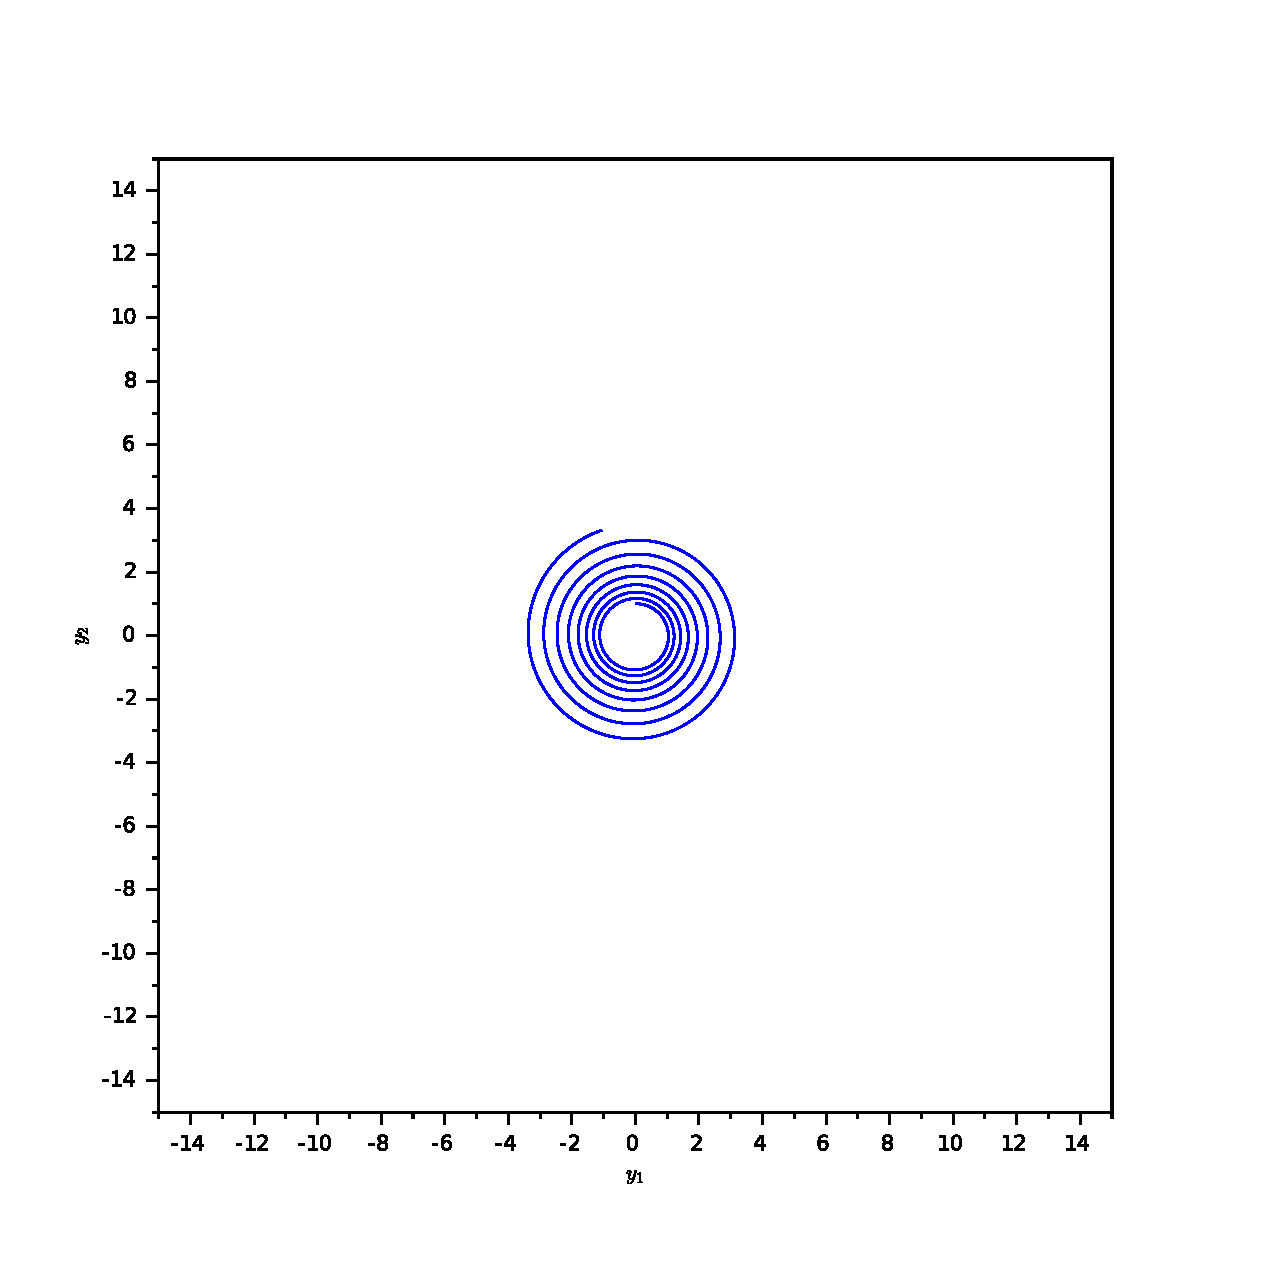
\includegraphics[width=0.3\textwidth]{images/soal_01_ode_euler_y1_y2.pdf}
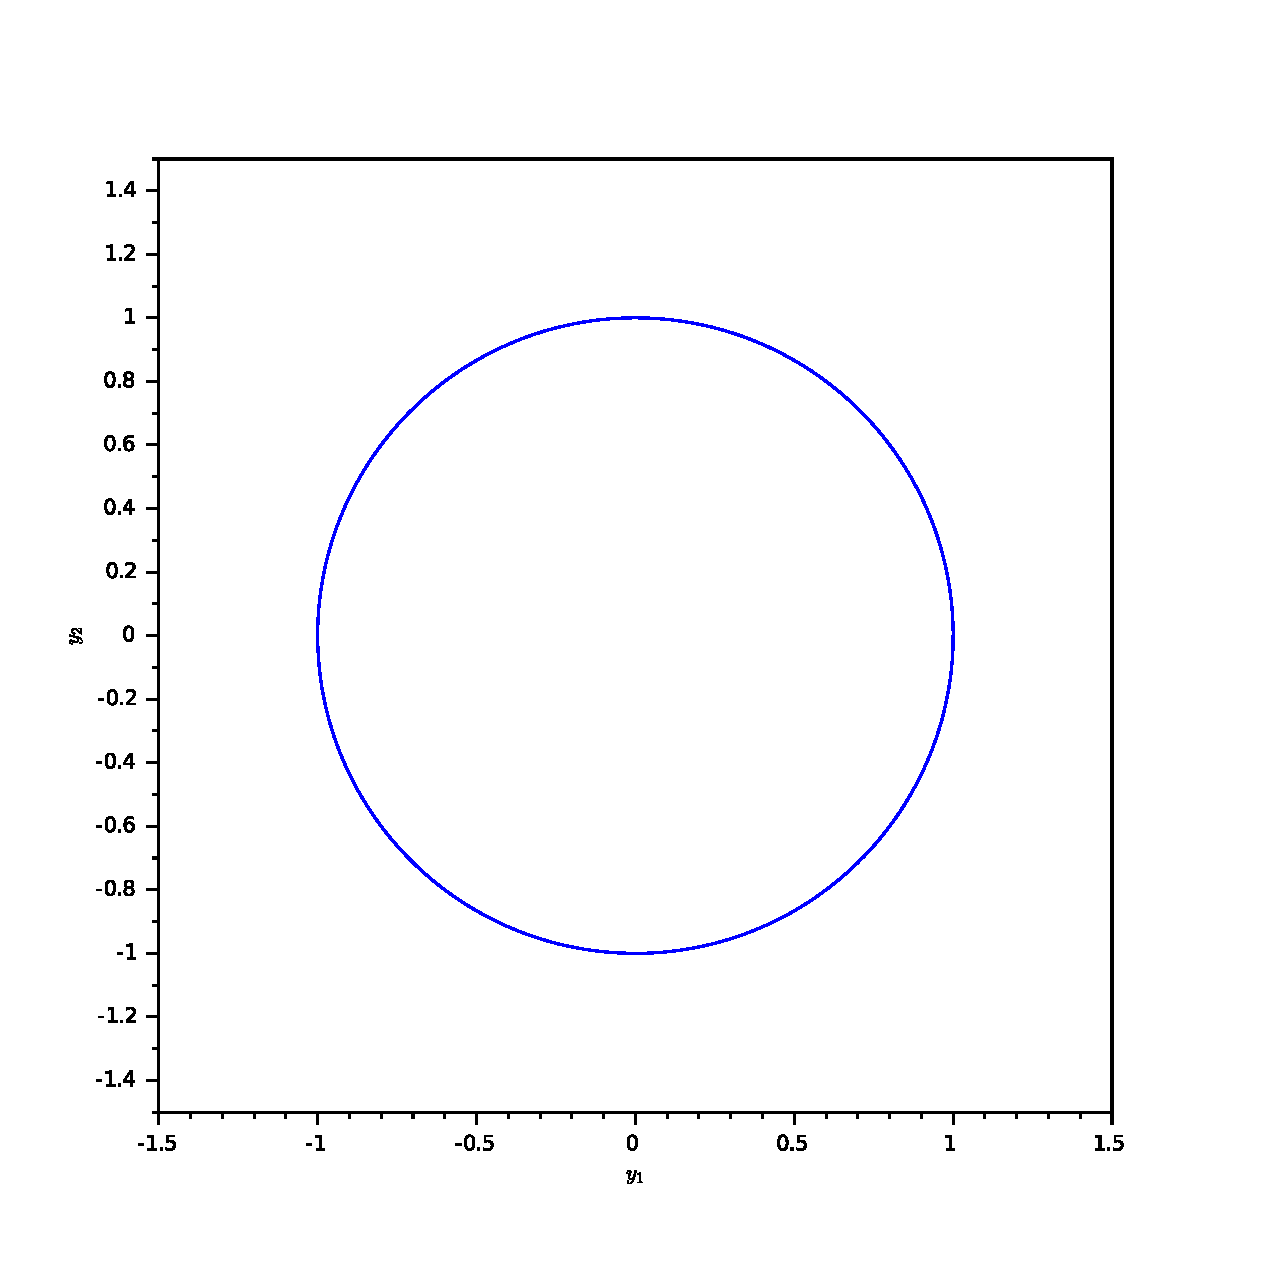
\includegraphics[width=0.3\textwidth]{images/soal_01_ode_euler_PC_y1_y2.pdf}
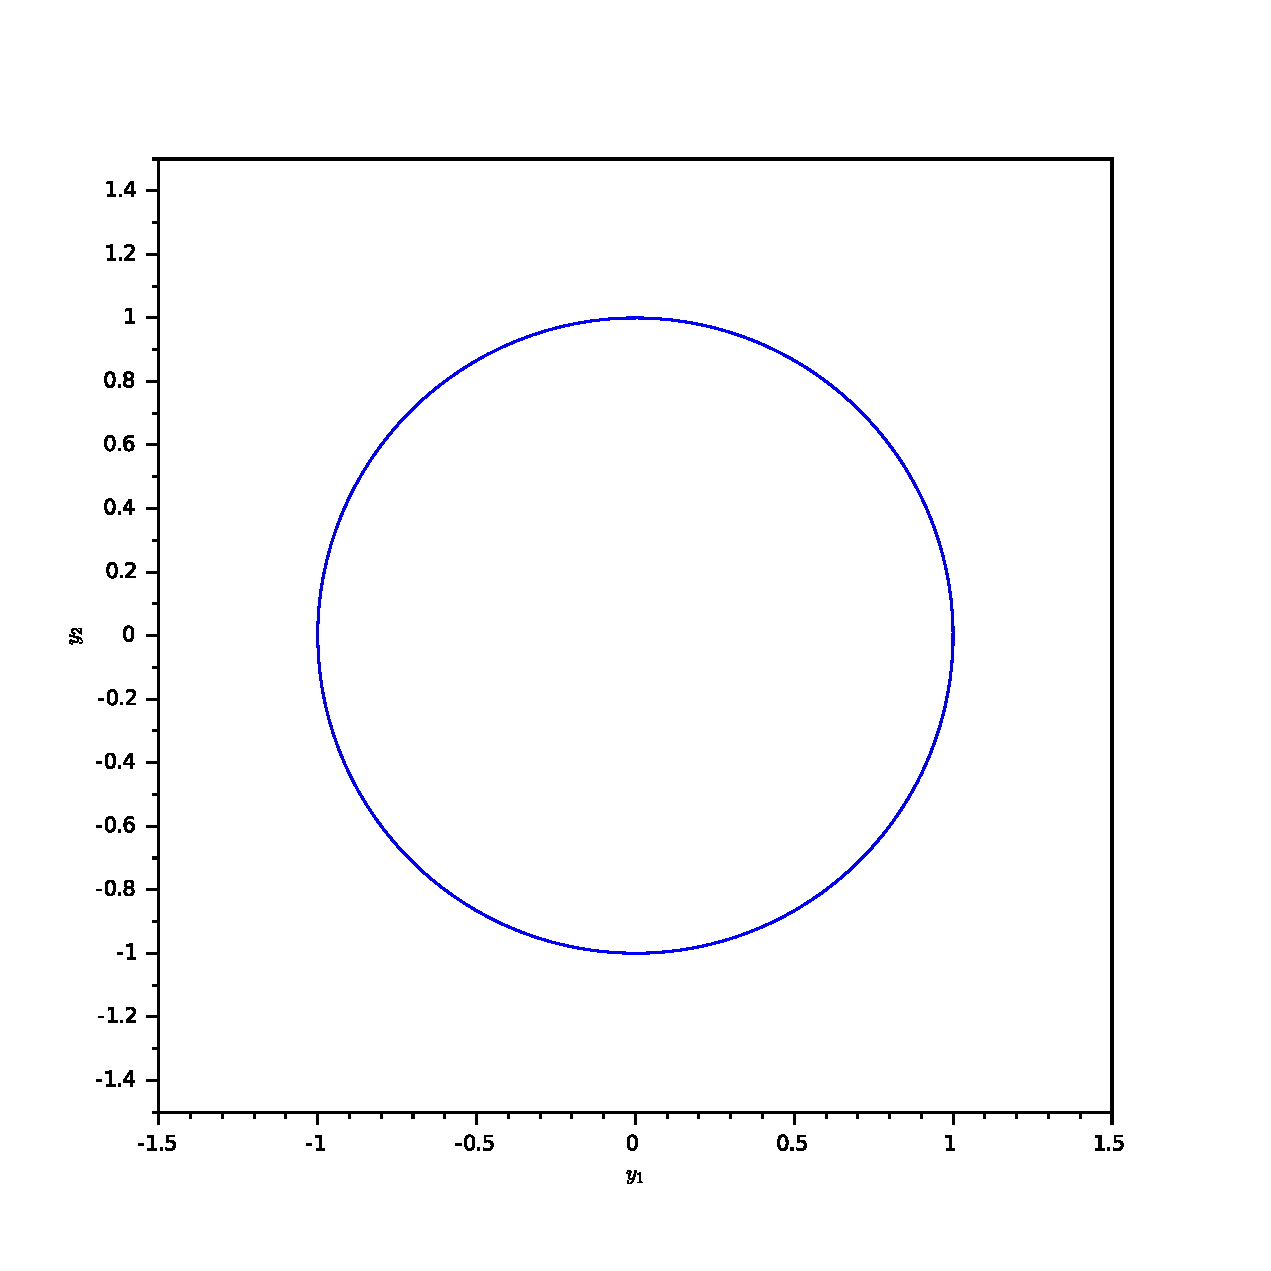
\includegraphics[width=0.3\textwidth]{images/soal_01_ode_RK4_y1_y2.pdf}
\par
\end{figure}

\begin{figure}[H]
\centering
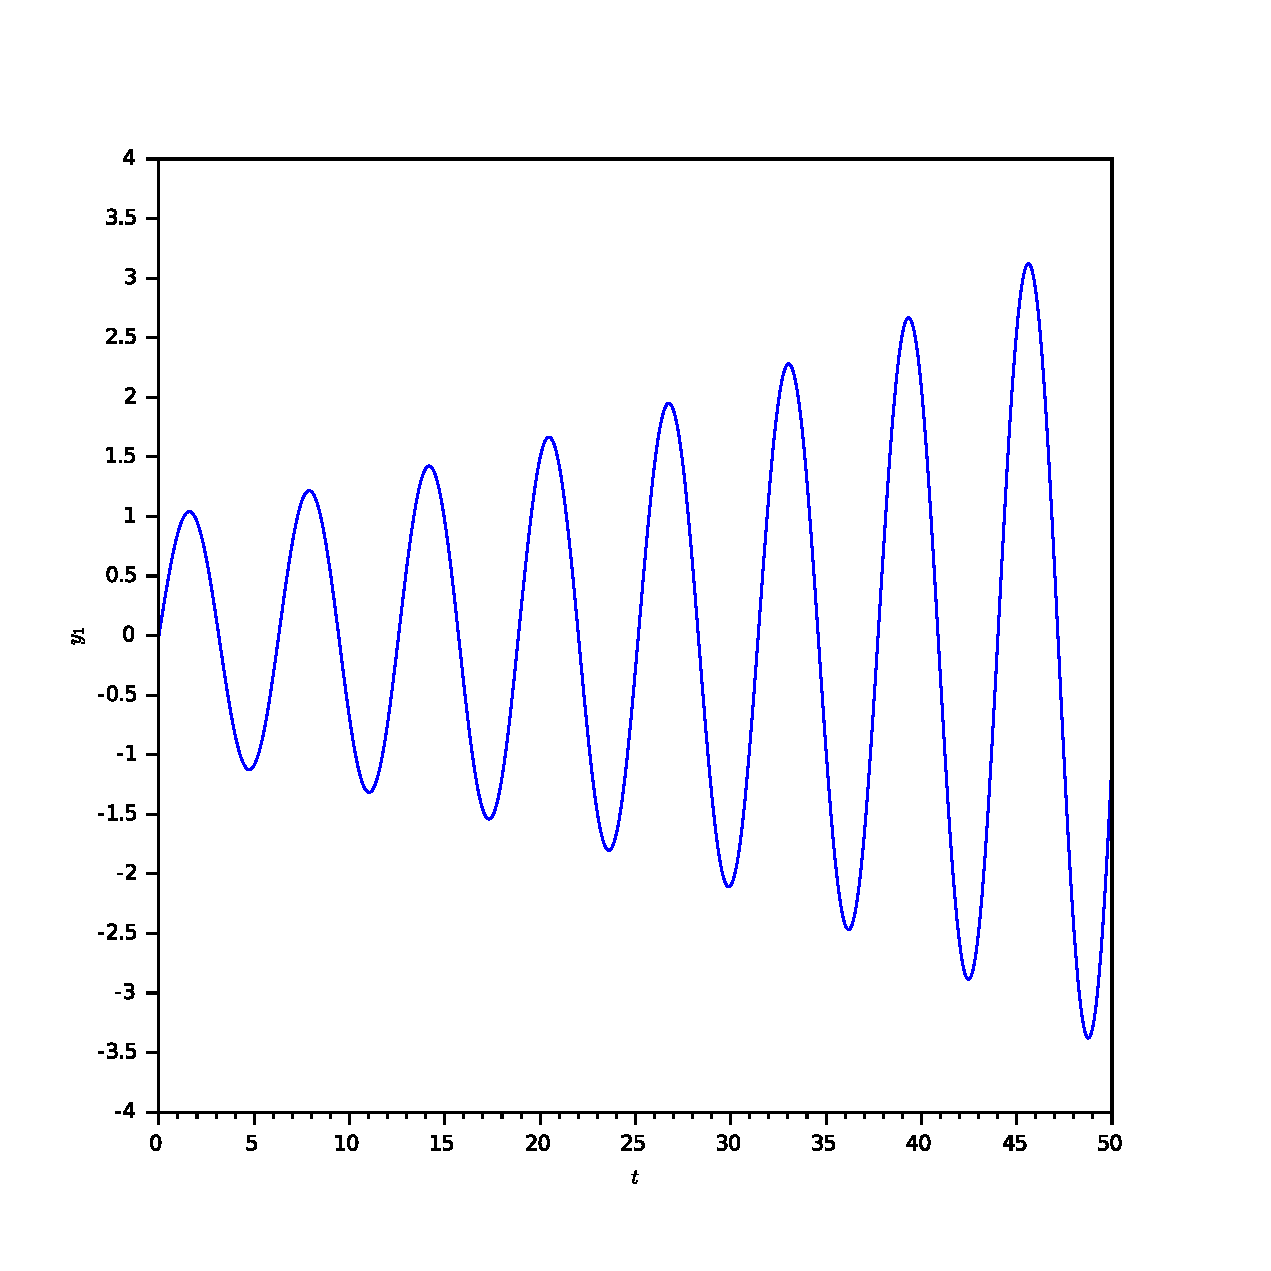
\includegraphics[width=0.3\textwidth]{images/soal_01_ode_euler_t_y1.pdf}
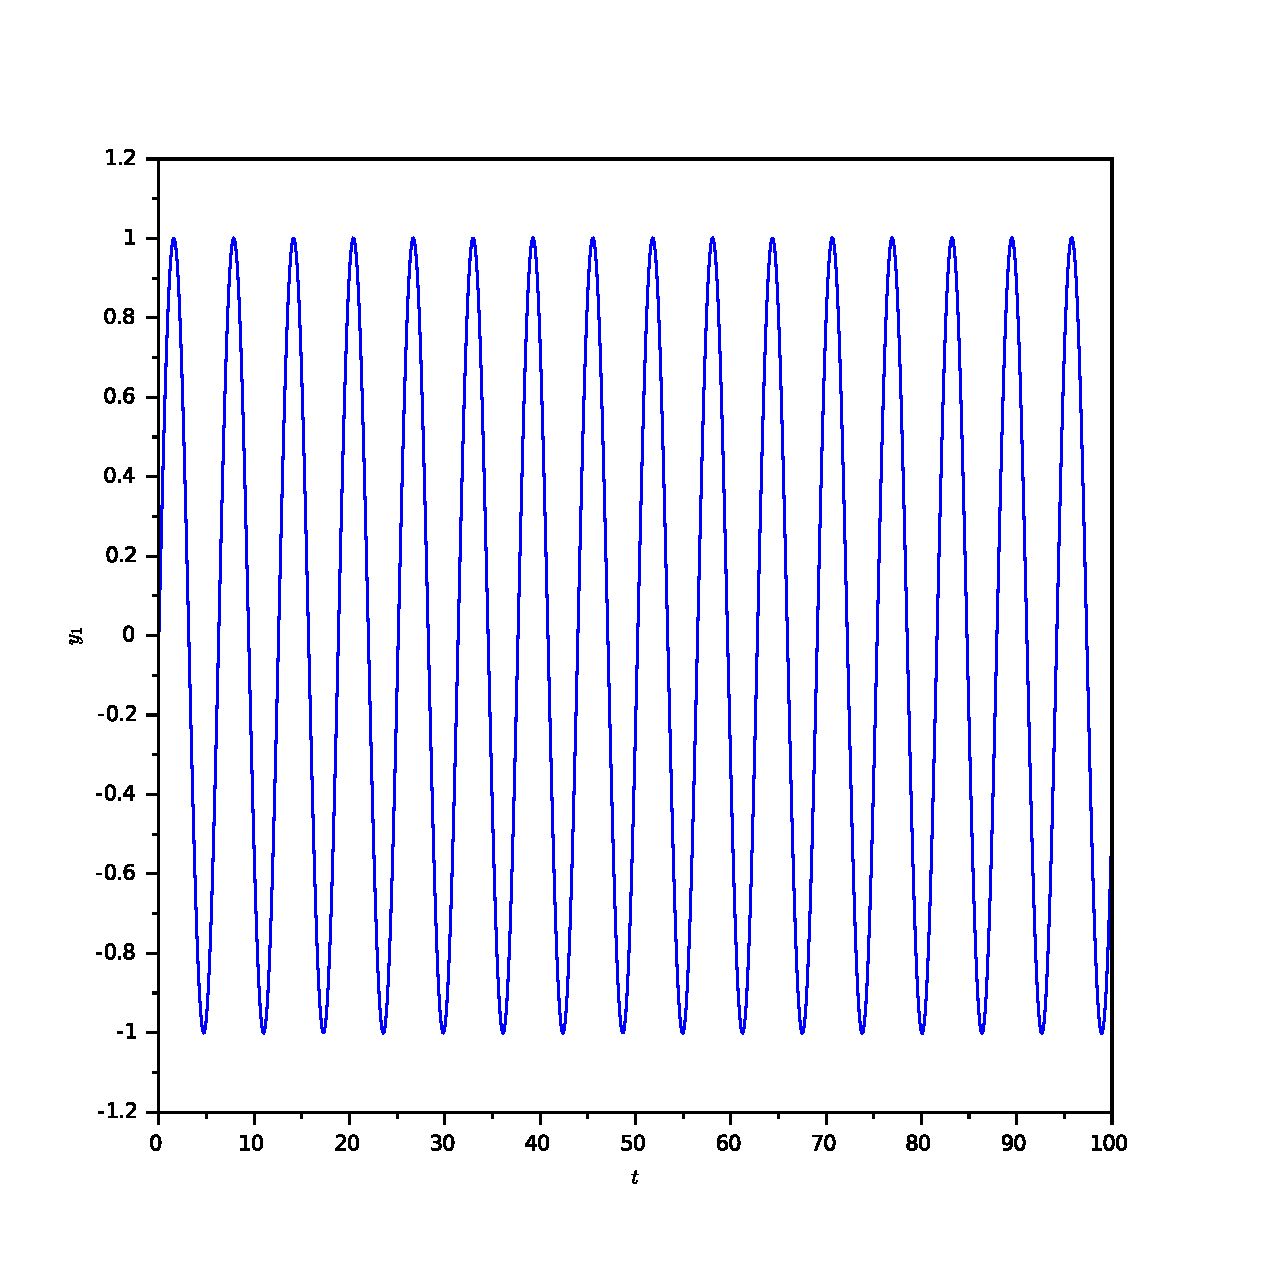
\includegraphics[width=0.3\textwidth]{images/soal_01_ode_euler_PC_t_y1.pdf}
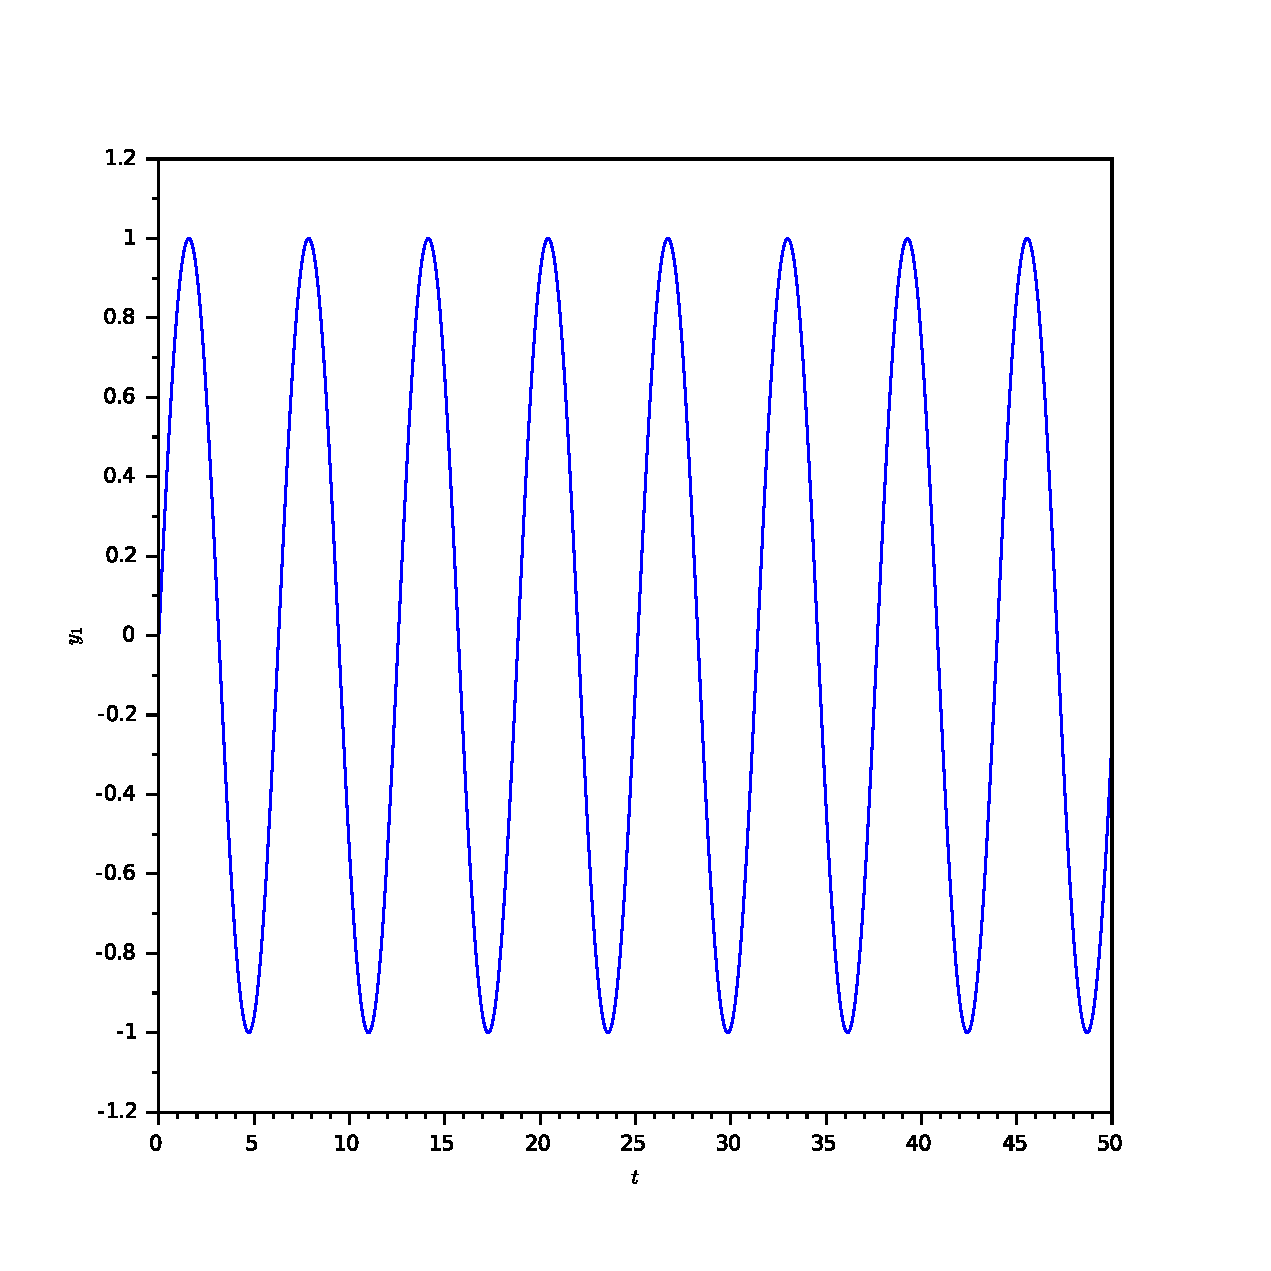
\includegraphics[width=0.3\textwidth]{images/soal_01_ode_RK4_t_y1.pdf}
\par
\end{figure}